\clearpage
\cleardoublepage

\chapter{激活函数}

\section{引言}

激活函数是应用于神经网络中每个神经元（或每层）输出的数学函数。它们向网络引入\textbf{非线性}，使其能够学习线性函数无法捕获的复杂模式。如果没有激活函数，无论网络有多少层，都只是执行线性变换，等同于一个线性层。

激活函数的选择会显著影响：
\begin{itemize}
    \item 网络学习复杂模式的能力
    \item 训练稳定性和收敛速度
    \item 反向传播过程中的梯度流动
    \item 神经元的输出范围
    \item 计算效率
\end{itemize}

本章将探讨各种激活函数的数学性质、优缺点和实际应用。

\section{为什么需要非线性？——通用逼近定理}

在逐一介绍激活函数之前，值得提出一个基本问题：\emph{为什么我们需要非线性激活函数？}答案在于神经网络理论中最著名的理论结果之一。

\subsection{定理}

\begin{定理}[通用逼近定理 \cite{hornik1991approximation}]
设 $\sigma$ 是一个非常数的、有界的、连续的激活函数。则对于任意连续函数 $g: [0,1]^n \to \mathbb{R}$ 和任意 $\epsilon > 0$，存在整数 $N > 0$、实常数 $\alpha_i, b_i \in \mathbb{R}$ 和实向量 $\mathbf{w}_i \in \mathbb{R}^n$，使得：
\begin{equation}
F(\mathbf{x}) = \sum_{i=1}^{N} \alpha_i \, \sigma\left(\mathbf{w}_i^\top \mathbf{x} + b_i\right)
\end{equation}
满足 $|F(\mathbf{x}) - g(\mathbf{x})| < \epsilon$ 对所有 $\mathbf{x} \in [0,1]^n$。
\end{定理}

\textbf{含义：}具有一个隐藏层和非多项式激活函数（包括 ReLU、sigmoid、tanh）的网络可以以任意精度逼近任何连续函数，只要神经元数量足够。

\subsection{直观解释}

考虑一个我们希望在1D区间上逼近的函数。隐藏层中的每个神经元通过 $\sigma(\mathbf{w}^\top \mathbf{x} + b)$ 计算一个"凸起"或"阶梯"函数，输出层用权重 $\alpha_i$ 将这些组合起来构建目标函数。神经元越多，逼近越精细：

\begin{figure}[htbp]
    \centering
    \begin{tikzpicture}[scale=0.9]
        \begin{axis}[
            xlabel=$x$,
            ylabel=$f(x)$,
            domain=0:1,
            samples=100,
            width=10cm,
            height=6cm,
            legend pos=north west
        ]
            % Target function
            \addplot[thick, black] {sin(deg(3*x)) * exp(-x)};
            \addlegendentry{目标函数 $g(x)$}
            % Approximation with 3 neurons
            \addplot[thick, blue, dashed] {max(0, 8*x - 2) + max(0, -8*x + 6)*0.8 + max(0, 5*x - 4)*0.3};
            \addlegendentry{3个神经元}
            % Approximation with more neurons
            \addplot[thick, red, densely dotted] {0.5*sin(deg(3*x))*exp(-x) + 0.3*sin(deg(6*x))*exp(-x) + 0.2*sin(deg(9*x))*exp(-x)};
            \addlegendentry{更多神经元（更好的拟合）}
        \end{axis}
    \end{tikzpicture}
    \caption[通用逼近的直观理解]{每个神经元贡献一个"凸起"或"阶梯"。更多神经元对目标函数产生更精细的逼近。}
    \label{fig:uat_intuition}
\end{figure}

\subsection{注意事项和实际意义}

通用逼近定理是一个\textbf{存在性}结果，而非\textbf{构造性}结果。它告诉我们存在一个合适的网络，但并未说明：
\begin{enumerate}
    \item \textbf{需要多少神经元}——对于高维函数，这个界是天文数字。
    \item \textbf{梯度下降能否找到它}——优化景观可能有糟糕的局部最小值。
    \item \textbf{更深的网络是否更高效}——Cybenko 和 Hornik 的结果适用于单隐藏层，但深度为组合函数提供了指数级的效率提升 \cite{montufar2014number}。
\end{enumerate}

在实践中，深度网络（多层、适度宽度）远远优于浅层、宽网络。关键洞察是：深度实现了\textbf{层次化特征组合}——每一层构建越来越抽象的表示。

\section{激活函数的历史发展}

了解激活函数的历史可以阐明为什么某些选择成为主流，以及该领域是如何演变的：

\begin{table}[ht]
    \centering
    \caption{激活函数发展历史时间表}
    \begin{tabular}{L{2cm} L{3cm} L{5.5cm} L{3cm}}
        \toprule
        \textbf{年份} & \textbf{函数} & \textbf{背景与动机} & \textbf{关键参考文献} \\
        \midrule
        1943 & 阈值（阶梯）函数 & McCulloch-Pitts神经元 & McCulloch \& Pitts \\
        1957 & 感知机 & 线性阈值单元 & Rosenblatt \\
        1960 & Adaline & 线性激活 + 符号 & Widrow \& Hoff \\
        1986 & Sigmoid & 可微分的反向传播 & Rumelhart et al. \\
        1991 & Tanh & 零中心化替代方案 & \\
        1998 & ReLU & 生物学的启发 & Hahnloser et al. \\
        2010 & Softmax & 概率多分类 & \\
        2011 & ReLU（复兴） & AlexNet：避免梯度消失 & \cite{krizhevsky2012imagenet} \\
        2015 & ELU, SELU & 平滑负区 & Clevert et al. \\
        2015 & PReLU & 可学习的负斜率 & He et al. \\
        2016 & Swish/SiLU & 自门控、非单调 & Ramachandran et al. \\
        2016 & GELU & 概率门控 & Hendrycks \& Gimpel \\
        2019 & Mish & 自正则化 & Misra \\
        2022 & StarReLU & 高效Transformer & Maulik et al. \\
        \bottomrule
    \end{tabular}
\end{table}

ReLU 的崛起故事尤其具有启发性。在2012年之前，sigmoid 和 tanh 是标准选择。然而，在深度网络中，这些饱和函数导致了\textbf{梯度消失}——通过 $L$ 个 sigmoid 导数的梯度乘积最多为 $(1/4)^L$，当 $L > 10$ 时变得可以忽略不计。AlexNet \cite{krizhevsky2012imagenet} 的突破表明，ReLU 的非饱和特性（$f'(x) = 1$ 当 $x > 0$）使得训练更深的网络成为可能，从根本上改变了这个领域。

\section{神经网络神经元}

在深入研究激活函数之前，让我们先了解它们在神经元中的作用。

单个人工神经元计算：
\begin{equation}
y = f(\mathbf{w}^\top \mathbf{x} + b) = f\left(\sum_{i=1}^{n} w_i x_i + b\right)
\end{equation}
其中：
\begin{itemize}
    \item $\mathbf{x} \in \mathbb{R}^n$ 是输入向量
    \item $\mathbf{w} \in \mathbb{R}^n$ 是权重向量
    \item $b \in \mathbb{R}$ 是偏置
    \item $f(\cdot)$ 是激活函数
    \item $y \in \mathbb{R}$ 是输出
\end{itemize}

\begin{figure}[htbp]
    \centering
    \begin{tikzpicture}[scale=0.9]
        % 输入节点
        \foreach \y/\label in {1/$x_1$, 2/$x_2$, 3/$\vdots$, 4/$x_n$} {
            \node[circle, draw=layer-input, fill=layer-input!30, minimum size=8mm] (x\y) at (0, 5-\y) {\label};
        }
        
        % 神经元
        \node[circle, draw=layer-hidden, fill=layer-hidden!30, minimum size=12mm, label=above:$f$] (neuron) at (4, 2.5) {$\sum + b$};
        
        % 输出
        \node[circle, draw=layer-output, fill=layer-output!30, minimum size=8mm] (y) at (7, 2.5) {$y$};
        
        % 连接
        \foreach \i in {1,...,4} {
            \draw[->, thick] (x\i) -- (neuron);
        }
        \draw[->, thick] (neuron) -- (y);
        
        % 权重标注
        \foreach \y/\w in {1/$w_1$, 2/$w_2$, 3/, 4/$w_n$} {
            \node[right] at (0.7, 4.5-\y) {\w};
        }
    \end{tikzpicture}
    \caption[单个神经元计算]{单个神经元计算加权和，然后应用激活函数}
    \label{fig:neuron}
\end{figure}

\section{线性激活函数}

虽然实际上不是严格的"激活函数"，但线性函数有时用于输出层。

\subsection{恒等函数}

\begin{equation}
f(x) = x
\end{equation}

\begin{itemize}
    \item \textbf{输出范围：}$(-\infty, \infty)$
    \item \textbf{导数：}$f'(x) = 1$
    \item \textbf{用例：}回归输出层
    \item \textbf{不推荐：}隐藏层（会使网络变为线性）
\end{itemize}

\section{Sigmoid 族}

Sigmoid 族激活函数将输入压缩到范围 $(0, 1)$，使其适用于二分类输出层。

\subsection{Sigmoid（逻辑斯蒂）}

\begin{equation}
\sigma(x) = \frac{1}{1 + e^{-x}} = \frac{e^x}{e^x + 1}
\end{equation}

\begin{properties}[Sigmoid的性质]
\begin{itemize}
    \item \textbf{输出范围：}$(0, 1)$
    \item \textbf{导数：}$\sigma'(x) = \sigma(x)(1 - \sigma(x))$
    \item \textbf{单调递增}
    \item \textbf{关于0.5对称}
    \item \textbf{处处光滑且可微分}
\end{itemize}
\end{properties}

\begin{figure}[htbp]
    \centering
    \begin{tikzpicture}[scale=0.9]
        \begin{axis}[
            xlabel=$x$,
            ylabel=$\sigma(x)$,
            domain=-6:6,
            samples=100,
            width=10cm,
            height=6cm,
            legend pos=north west
        ]
            \addplot[thick, blue] {1/(1 + exp(-x))};
            \addlegendentry{Sigmoid $\sigma(x)$}
            \addplot[thick, red, dashed] {exp(-x)/(1 + exp(-x))^2};
            \addlegendentry{导数 $\sigma'(x)$}
            
            % y=0.5的水平线
            \addplot[gray, dashed] {0.5};
            
            % y=0和y=1的水平线
            \addplot[gray, dotted] {1};
            \addplot[gray, dotted] {0};
        \end{axis}
    \end{tikzpicture}
    \caption[Sigmoid函数及其导数]{Sigmoid函数及其导数}
    \label{fig:sigmoid}
\end{figure}

\begin{advantages}
    \item 平滑的梯度
    \item 输出可以解释为概率
    \item 历史上广泛使用
\end{advantages}

\begin{disadvantages}
    \item \textbf{梯度消失：}对于大的 $|x|$，$\sigma'(x) \approx 0$
    \item \textbf{非零中心化：}输出总是正的
    \item \textbf{指数计算：}比简单函数慢
    \item \textbf{饱和：}在0和1处饱和
\end{disadvantages}

\subsubsection{数学分析：为什么 Sigmoid 导致梯度消失}

考虑一个每层都使用 sigmoid 激活的 $L$ 层网络。在反向传播过程中，流经第 $l$ 层的梯度乘以每个中间层的导数：
\begin{equation}
\frac{\partial \mathcal{L}}{\partial z_1} = \underbrace{\frac{\partial \mathcal{L}}{\partial z_L}}_{\text{输出梯度}} \cdot \prod_{l=2}^{L} \underbrace{\frac{\partial a_l}{\partial z_l}}_{= \sigma'(z_l)} \cdot \underbrace{\frac{\partial z_l}{\partial a_{l-1}}}_{= \mathbf{W}_l}
\end{equation}

由于 $\sigma'(z) = \sigma(z)(1-\sigma(z)) \leq \frac{1}{4}$（在 $z=0$ 处最大），sigmoid 导数分量单独提供一个最多为 $(1/4)^{L-1}$ 的乘数因子：
\begin{equation}
\left\|\frac{\partial \mathcal{L}}{\partial z_1}\right\| \leq \left(\frac{1}{4}\right)^{L-1} \cdot \prod_{l=2}^{L} \|\mathbf{W}_l\| \cdot \left\|\frac{\partial \mathcal{L}}{\partial z_L}\right\|
\end{equation}

对于50层网络：$(1/4)^{49} \approx 10^{-30}$。即使权重范数适中，梯度也有效地消失了。这个数学分析解释了为什么比几层更深的 sigmoid 网络在采用替代激活函数之前基本上是不可训练的。

\subsubsection{导数推导}

从 $\sigma(x) = \frac{1}{1 + e^{-x}}$ 开始：
\begin{align}
\sigma'(x) &= \frac{d}{dx}\left((1 + e^{-x})^{-1}\right) = (1 + e^{-x})^{-2} \cdot e^{-x} \\
&= \frac{1}{1 + e^{-x}} \cdot \frac{e^{-x}}{1 + e^{-x}} \\
&= \sigma(x) \cdot (1 - \sigma(x))
\end{align}
这种优雅的形式意味着梯度可以直接从输出计算，无需再次求值指数。最大值 $\sigma'(0) = 0.25$ 出现在 $x = 0$ 处。

\begin{example}[二分类中的Sigmoid]
对于二分类，sigmoid 输出可以解释为：
\begin{equation}
P(y=1|\mathbf{x}) = \sigma(\mathbf{w}^\top \mathbf{x} + b)
\end{equation}
带 sigmoid 的交叉熵损失为：
\begin{equation}
\mathcal{L} = -[y \log \hat{y} + (1-y) \log(1-\hat{y})]
\end{equation}
其中 $\hat{y} = \sigma(\mathbf{w}^\top \mathbf{x} + b)$。
\end{example}

\subsection{双曲正切（Tanh）}

\begin{equation}
\tanh(x) = \frac{e^x - e^{-x}}{e^x + e^{-x}} = 2\sigma(2x) - 1
\end{equation}

\begin{properties}[Tanh的性质]
\begin{itemize}
    \item \textbf{输出范围：}$(-1, 1)$
    \item \textbf{导数：}$\tanh'(x) = 1 - \tanh^2(x)$
    \item \textbf{零中心化输出}
    \item \textbf{单调递增}
\end{itemize}
\end{properties}

\begin{figure}[htbp]
    \centering
    \begin{tikzpicture}[scale=0.9]
        \begin{axis}[
            xlabel=$x$,
            ylabel=$\tanh(x)$,
            domain=-6:6,
            samples=100,
            width=10cm,
            height=6cm,
            legend pos=south east
        ]
            \addplot[thick, blue] {tanh(x)};
            \addlegendentry{Tanh $\tanh(x)$}
            \addplot[thick, red, dashed] {1/(cosh(x)^2)};
            \addlegendentry{导数 $\tanh'(x)$}
            
            % 水平线
            \addplot[gray, dashed] {0};
            \addplot[gray, dotted] {1};
            \addplot[gray, dotted] {-1};
        \end{axis}
    \end{tikzpicture}
    \caption[Tanh函数及其导数]{Tanh函数及其导数}
    \label{fig:tanh}
\end{figure}

\begin{advantages}
    \item 零中心化输出（更强的梯度）
    \item 比 sigmoid 更强的梯度
    \item 输出在 $(-1, 1)$，通常对隐藏层更好
\end{advantages}

\begin{disadvantages}
    \item \textbf{梯度消失：}对于大的 $|x|$ 仍然存在
    \item \textbf{指数计算}
    \item \textbf{在 $\pm 1$ 处饱和}
\end{disadvantages}

\section{修正线性单元（ReLU）族}

ReLU 族由于其计算效率和训练深度网络的有效性，已成为现代深度学习中隐藏层的主流选择。

\subsection{ReLU}

\begin{equation}
\text{ReLU}(x) = \max(0, x) = 
\begin{cases}
x & \text{如果 } x > 0 \\
0 & \text{如果 } x \leq 0
\end{cases}
\end{equation}

\begin{properties}[ReLU的性质]
\begin{itemize}
    \item \textbf{输出范围：}$[0, \infty)$
    \item \textbf{导数：} 
    \begin{equation}
    \text{ReLU}'(x) = 
    \begin{cases}
    1 & \text{如果 } x > 0 \\
    0 & \text{如果 } x \leq 0
    \end{cases}
    \end{equation}
    \item \textbf{计算高效}
    \item \textbf{稀疏激活}
\end{itemize}
\end{properties}

\begin{figure}[htbp]
    \centering
    \begin{tikzpicture}[scale=0.9]
        \begin{axis}[
            xlabel=$x$,
            ylabel=$\text{ReLU}(x)$,
            domain=-4:4,
            samples=100,
            width=10cm,
            height=6cm,
            legend pos=north west
        ]
            \addplot[thick, blue] {max(0, x)};
            \addlegendentry{ReLU}
            \addplot[thick, red, dashed, domain=0:4] {1};
            \addlegendentry{导数}
            
            % x=0处的垂直线
            \addplot[const plot, thick, blue, domain=-4:0] {0};
        \end{axis}
    \end{tikzpicture}
    \caption[ReLU函数及其导数]{ReLU函数及其导数}
    \label{fig:relu}
\end{figure}

\begin{advantages}
    \item \textbf{计算非常快}
    \item \textbf{减少正激活的梯度消失问题}
    \item \textbf{稀疏表示：}并非所有神经元同时激活
    \item \textbf{在深度网络中表现优异}
    \item \textbf{生物学合理性}
\end{advantages}

\subsubsection{为什么ReLU防止梯度消失：数学分析}

ReLU 相对于 sigmoid 的关键优势是其\textbf{非饱和}特性。对于任何预激活 $z_l > 0$ 的神经元：
\begin{equation}
\text{ReLU}'(z_l) = 1 \quad \text{（无衰减）}
\end{equation}

在使用 ReLU 激活的深度网络中，"活跃"路径的梯度为：
\begin{equation}
\frac{\partial \mathcal{L}}{\partial z_1} = \frac{\partial \mathcal{L}}{\partial z_L} \cdot \prod_{l=2}^{L} \mathbf{1}_{\{z_l > 0\}} \cdot \mathbf{W}_l
\end{equation}
指示函数 $\mathbf{1}_{\{z_l > 0\}}$ 要么是0要么是1——没有指数衰减。如果每层大约一半神经元是活跃的，梯度幅度为：
\begin{equation}
\left\|\frac{\partial \mathcal{L}}{\partial z_1}\right\| \approx \left(\frac{1}{2}\right)^{L-1} \cdot \prod_{l=2}^{L} \|\mathbf{W}_l\| \cdot \left\|\frac{\partial \mathcal{L}}{\partial z_L}\right\|
\end{equation}

虽然因子 $(1/2)^{L-1}$ 仍然指数衰减，但在实践中通过以下方式缓解：
\begin{itemize}
    \item \textbf{He初始化} \cite{he2015delving}：将权重方差设置为 $2/n_{\text{in}}$ 以补偿预期的不活跃神经元比例。
    \item \textbf{残差连接} \cite{he2016deep}：跳跃连接提供了一条绕过乘法衰减的替代梯度路径（第6章）。
    \item \textbf{批归一化} \cite{ioffe2015batch}：稳定激活的分布，保持它们在非饱和区域。
\end{itemize}

\subsubsection{ReLU、稀疏性与生物学动机}

ReLU 的 $\max(0, x)$ 操作创建稀疏激活：对于典型的初始化，大约 50\% 的神经元输出为零。这种稀疏性有几个好处：
\begin{enumerate}
    \item \textbf{信息解耦：}稀疏表示往往更易解释和鲁棒（类似于神经科学中的稀疏编码）。
    \item \textbf{效率：}零值神经元对下游计算没有贡献，支持硬件优化。
    \item \textbf{生物学合理性：}生物神经元表现出阈值行为——只有当输入超过阈值时才发放。ReLU 定性地捕获了这一点，不像平滑的 sigmoid。
\end{enumerate}

\begin{disadvantages}
    \item \textbf{死亡ReLU问题：}如果神经元的权重更新使得 $\mathbf{w}^\top \mathbf{x} + b \leq 0$ 对所有输入，该神经元将永远输出零。
    \item \textbf{非零中心化}
    \item \textbf{输出无界}
\end{disadvantages}

\begin{note}[死亡ReLU问题]
如果神经元的权重更新使得 $\mathbf{w}^\top \mathbf{x} + b \leq 0$ 对所有输入，该神经元将永远输出零。这被称为"死亡ReLU"或"死神经元"问题。当输入为负时梯度为零，神经元停止学习。

解决方案包括：
\begin{itemize}
    \item Leaky ReLU
    \item PReLU
    \item ELU
    \item 正确的权重初始化
    \item 较低的学习率
\end{itemize}
\end{note}

\subsection{Leaky ReLU}

\begin{equation}
\text{LeakyReLU}(x) = 
\begin{cases}
x & \text{如果 } x > 0 \\
\alpha x & \text{如果 } x \leq 0
\end{cases}
= \max(0, x) + \alpha \min(0, x)
\end{equation}
其中 $\alpha$ 是一个小的正常数（通常 $\alpha = 0.01$）。

\begin{properties}[Leaky ReLU的性质]
\begin{itemize}
    \item \textbf{输出范围：}$(-\infty, \infty)$
    \item \textbf{导数：} 
    \begin{equation}
    \text{LeakyReLU}'(x) = 
    \begin{cases}
    1 & \text{如果 } x > 0 \\
    \alpha & \text{如果 } x \leq 0
    \end{cases}
    \end{equation}
    \item \textbf{允许小的负值}
\end{itemize}
\end{properties}

\begin{advantages}
    \item \textbf{没有死亡ReLU问题}
    \item \textbf{允许小的负梯度}
    \item \textbf{近似零中心化}
\end{advantages}

\begin{disadvantages}
    \item 超参数 $\alpha$ 需要调整
    \item 性能可能不会显著优于 ReLU
\end{disadvantages}

\subsection{参数化ReLU（PReLU）}

\begin{equation}
\text{PReLU}(x) = 
\begin{cases}
x & \text{如果 } x > 0 \\
\alpha x & \text{如果 } x \leq 0
\end{cases}
\end{equation}
其中 $\alpha$ 是一个可学习参数（可以是每通道的）。

\begin{note}
PReLU 允许网络学习负值的最佳斜率，可能提高性能。
\end{note}

\subsection{指数线性单元（ELU）}

\begin{equation}
\text{ELU}(x) = 
\begin{cases}
x & \text{如果 } x > 0 \\
\alpha(e^x - 1) & \text{如果 } x \leq 0
\end{cases}
\end{equation}
其中 $\alpha > 0$ 是一个超参数。

\begin{properties}[ELU的性质]
\begin{itemize}
    \item \textbf{输出范围：}$(-\alpha, \infty)$
    \item \textbf{对于 $x < 0$ 平滑}
    \item \textbf{负值使均值更接近零}
\end{itemize}
\end{properties}

\begin{figure}[htbp]
    \centering
    \begin{tikzpicture}[scale=0.9]
        \begin{axis}[
            xlabel=$x$,
            ylabel=激活值,
            domain=-4:4,
            samples=100,
            width=10cm,
            height=6cm,
            legend pos=north west
        ]
            \addplot[thick, blue] {max(0, x)};
            \addlegendentry{ReLU}
            \addplot[thick, green] {max(0, x) + 0.01*min(0, x)};
            \addlegendentry{LeakyReLU}
            \addplot[thick, red] {x > 0 ? x : 1.0*(exp(x) - 1)};
            \addlegendentry{ELU}
        \end{axis}
    \end{tikzpicture}
    \caption[ReLU变体比较]{ReLU及其变体的比较}
    \label{fig:relu_variants}
\end{figure}

\begin{advantages}
    \item \textbf{没有死亡ReLU问题}
    \item \textbf{输出更接近零均值}
    \item \textbf{更平滑的梯度}
\end{advantages}

\begin{disadvantages}
    \item 负值的指数计算
    \item 前向传播较慢
\end{disadvantages}

\subsection{Swish / SiLU}

\begin{equation}
\text{Swish}(x) = x \cdot \sigma(x) = \frac{x}{1 + e^{-x}}
\end{equation}

Swish 已成为深度网络中 ReLU 的广泛使用的平滑替代方案 \cite{ramachandran2017searching}。

\begin{properties}[Swish的性质]
\begin{itemize}
    \item \textbf{输出范围：}大约 $(-0.31, \infty)$
    \item \textbf{自门控}
    \item \textbf{非单调}（对于小的负值有凹陷）
    \item \textbf{导数：}$\text{Swish}'(x) = \sigma(x) + x \cdot \sigma(x)(1 - \sigma(x)) = \text{Swish}(x) + \sigma(x)(1 - \text{Swish}(x))$
\end{itemize}
\end{properties}

\begin{figure}[htbp]
    \centering
    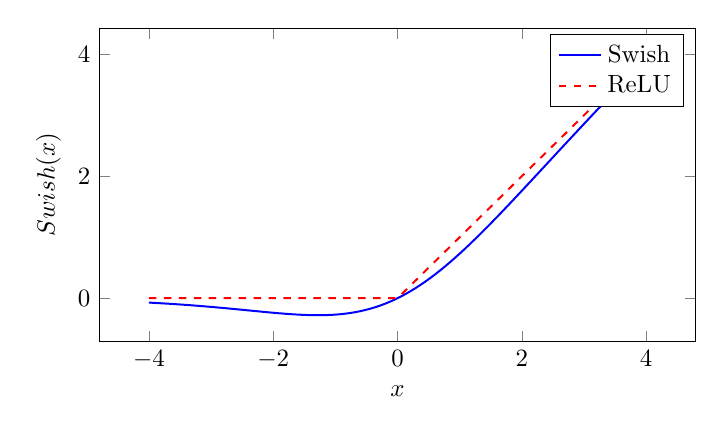
\begin{tikzpicture}[scale=0.9]
        \begin{axis}[
            xlabel=$x$,
            ylabel=$\text{Swish}(x)$,
            domain=-4:4,
            samples=100,
            width=10cm,
            height=6cm
        ]
            \addplot[thick, blue] {x / (1 + exp(-x))};
            \addlegendentry{Swish}
            \addplot[thick, red, dashed] {max(0, x)};
            \addlegendentry{ReLU}
        \end{axis}
    \end{tikzpicture}
    \caption[Swish激活函数]{Swish vs ReLU}
    \label{fig:swish}
\end{figure}

\subsection{Mish}

Mish \cite{misra2019mish} 是一个自正则化的非单调激活函数：
\begin{equation}
\text{Mish}(x) = x \cdot \tanh(\text{softplus}(x)) = x \cdot \tanh(\ln(1 + e^x))
\end{equation}

\begin{properties}[Mish的性质]
\begin{itemize}
    \item \textbf{输出范围：}大约 $(-0.308, \infty)$（下方有界，上方无界）
    \item \textbf{非单调：}类似于 Swish，对负的 $x$ 略有凹陷
    \item \textbf{处处光滑：}无限可微（$C^\infty$）
    \item \textbf{自正则化：}非单调形状作为隐式正则化器
\end{itemize}
\end{properties}

导数是：
\begin{equation}
\text{Mish}'(x) = \frac{e^x \cdot (4(e^x + 2)) + 4x \cdot e^{2x} + 2 \cdot e^{3x} + x \cdot e^{4x} + 2}{(2e^x + 2)^2}
\end{equation}

虽然导数很复杂，但关键洞察是 Mish 始终保持正梯度（像 ReLU），但对于负输入有更平滑、有界的梯度，提供温和的正则化。在经验上，Mish 在图像分类基准测试（ImageNet、CIFAR-10/100）和目标检测任务上始终匹配或优于 ReLU 和 Swish。

\begin{advantages}
    \item 在视觉任务上比 ReLU/Swish 表现更强
    \item 平滑、非单调形状提供隐式正则化
    \item 无需额外超参数
\end{advantages}

\begin{disadvantages}
    \item 计算更昂贵（$\tanh$ + softplus）
    \item 导数公式复杂
\end{disadvantages}

\subsection{StarReLU}

StarReLU，在 \cite{maulik2024starrelu} 中引入，是一种专为 transformer 设计的新型自门控激活函数：
\begin{equation}
\text{StarReLU}(x) = s \cdot \text{ReLU}(x)^2 + \beta
\end{equation}
其中 $s$ 和 $\beta$ 是可学习参数（初始化为 $s = 1, \beta = 0$）。

\textbf{动机：}在 transformer 中，计算瓶颈是应用于 $N \times d$ 隐藏状态张量每个元素的激活函数。StarReLU 的二次形式 $\text{ReLU}(x)^2$ 比 GELU/Swish 更简单（无 $\tanh$ 或 $\sigma$），同时提供：
\begin{itemize}
    \item \textbf{自门控：}平方运算自然地将负输入归零。
    \item \textbf{可学习的尺度和偏移：}$s$ 和 $\beta$ 调整激活范围。
    \item \textbf{计算效率：}在 transformer 块中比 GELU 减少 60\% 的 FLOPs，没有精度损失。
\end{itemize}

StarReLU 代表了设计\textbf{硬件感知}激活函数的趋势——利用这样一个事实：在现代硬件上，简单操作（乘法、加法）比超越函数（exp、tanh、erf）便宜得多。

\subsection{GELU（高斯误差线性单元）}

\begin{equation}
\text{GELU}(x) = x \cdot \Phi(x)
\end{equation}
其中 $\Phi(x)$ 是标准正态分布的累积分布函数：
\begin{equation}
\Phi(x) = \frac{1}{2}\left[1 + \text{erf}\left(\frac{x}{\sqrt{2}}\right)\right]
\end{equation}

一个计算高效的近似：
\begin{equation}
\text{GELU}(x) \approx \frac{x}{2} \cdot \left(1 + \tanh\left(\sqrt{\frac{2}{\pi}}\left(x + 0.044715x^3\right)\right)\right)
\end{equation}

GELU 用于 BERT、GPT 和许多 transformer 架构。

\subsubsection{概率解释：GELU、Dropout和高斯CDF}

GELU 函数有一个连接它与 dropout \cite{clark2022unified} 的深层概率解释。考虑一个随机神经元，其中输入 $x$ 乘以随机伯努利掩码 $m \sim \text{Bernoulli}(\Phi(x))$：
\begin{equation}
y = x \cdot m, \quad P(m = 1 \mid x) = \Phi(x)
\end{equation}
这个随机神经元的期望输出为：
\begin{equation}
\mathbb{E}[y \mid x] = x \cdot \Phi(x) = \text{GELU}(x)
\end{equation}

\textbf{关键洞察：}GELU 是一个随机门控神经元的\textbf{确定性期望}，其中门控概率等于高斯 CDF。这提供了一种统一视图：
\begin{itemize}
    \item \textbf{Dropout} 以与输入无关的概率 $p$ 随机将激活置零。
    \item \textbf{GELU} 根据激活幅度自适应地门控激活（与输入相关）。
    \item 两者都可以看作乘性噪声，但 GELU 的噪声是\textbf{自适应的}——较大的输入更可能通过。
\end{itemize}

这个解释解释了为什么 GELU 在 transformer 中效果这么好：它提供了一种依赖于输入幅度的平滑、"软"版本的 dropout，提供隐式正则化，而不像注意力机制中随机 dropout 那样有训练不稳定性。

\subsubsection{GELU的导数}

从 $\text{GELU}(x) = x\Phi(x)$，通过乘积规则：
\begin{equation}
\text{GELU}'(x) = \Phi(x) + x\phi(x)
\end{equation}
其中 $\phi(x) = \frac{1}{\sqrt{2\pi}}e^{-x^2/2}$ 是标准正态分布的概率密度函数。注意 $\text{GELU}'(x) > 0$ 对所有 $x$（函数严格递增），但 $\text{GELU}'(x) < 1$（不像 ReLU），提供自然的梯度缩放。

\begin{properties}[GELU的性质]
\begin{itemize}
    \item \textbf{与dropout结合时是随机正则化器}
    \item \textbf{在所有区域非线性}
    \item \textbf{大约等于：}$0.5x(1 + \tanh(\sqrt{2/\pi}(x + 0.044715x^3)))$
    \item \textbf{零中心化输出}
\end{itemize}
\end{properties}

\begin{advantages}
    \item Transformer 中的最先进性能
    \item 结合了 ReLU 和 dropout 的优点
    \item 平滑且非单调
\end{advantages}

\section{特殊激活函数}

\subsection{Softmax}

\begin{equation}
\text{softmax}(x_i) = \frac{e^{x_i}}{\sum_{j=1}^{K} e^{x_j}} \quad \text{对于 } i = 1, \ldots, K
\end{equation}

Softmax 用于多分类输出层。

\begin{properties}[Softmax的性质]
\begin{itemize}
    \item \textbf{输出范围：}每个输出在 $(0, 1)$
    \item \textbf{求和约束：}$\sum_i \text{softmax}(x_i) = 1$
    \item \textbf{概率解释}
    \item \textbf{平移不变：}对于任意常数 $c$，$\text{softmax}(x + c) = \text{softmax}(x)$
\end{itemize}
\end{properties}

\begin{advantages}
    \item 输出是有效的概率分布
    \item 支持交叉熵损失优化
    \item 自然处理多分类
\end{advantages}

\begin{disadvantages}
    \item 仅用于输出层（不是隐藏层）
    \item 当logits非常大时可能饱和
\end{disadvantages}

\begin{note}[实践中的Softmax]
为数值稳定性，实现 softmax 为：
\begin{equation}
\text{softmax}(x_i) = \frac{e^{x_i - \max(x)}}{\sum_j e^{x_j - \max(x)}}
\end{equation}
这减去最大值以防止指数溢出。
\end{note}

\section{选择激活函数}

激活函数的选择取决于具体任务和网络架构。以下是一般指南：

\begin{table}[ht]
    \centering
    \caption{激活函数选择指南}
    \begin{tabular}{L{3cm} L{5cm} L{4cm}}
        \toprule
        \textbf{层类型} & \textbf{推荐函数} & \textbf{注意事项} \\
        \midrule
        \textbf{隐藏层（通用）} & ReLU, GELU & ReLU 是默认选择 \\
        \textbf{隐藏层（深度）} & ReLU, GELU, ELU & 避免深度网络中的 sigmoid/tanh \\
        \textbf{隐藏层（CNN）} & ReLU, GELU & 医学成像用 LeakyReLU \\
        \textbf{隐藏层（RNN）} & Tanh & RNN 的通常默认选择 \\
        \textbf{隐藏层（Transformer）} & GELU & 用于 BERT、GPT 等 \\
        \textbf{输出（二分类）} & Sigmoid & 用于概率输出 \\
        \textbf{输出（多分类）} & Softmax & 用于概率分布 \\
        \textbf{输出（回归）} & 恒等函数 / 无 & 用于无界输出 \\
        \textbf{输出（有界）} & Sigmoid, Tanh & 用于 $[0,1]$ 或 $[-1,1]$ 输出 \\
        \bottomrule
    \end{tabular}
\end{table}

\begin{figure}[htbp]
    \centering
    \begin{tikzpicture}[scale=0.8]
        \begin{axis}[
            xlabel=$x$,
            ylabel=激活值,
            domain=-4:4,
            samples=100,
            width=14cm,
            height=8cm,
            legend pos=north east
        ]
            \addplot[thick, blue] {1/(1 + exp(-x))};
            \addlegendentry{Sigmoid}
            \addplot[thick, green] {tanh(x)};
            \addlegendentry{Tanh}
            \addplot[thick, red] {max(0, x)};
            \addlegendentry{ReLU}
            \addplot[thick, purple] {x / (1 + exp(-x))};
            \addlegendentry{Swish}
            \addplot[thick, orange] {x > 0 ? x : 1.0*(exp(x) - 1)};
            \addlegendentry{ELU}
        \end{axis}
    \end{tikzpicture}
    \caption[各种激活函数比较]{各种激活函数的比较}
    \label{fig:activation_comparison}
\end{figure}

\section{实践注意事项}

\subsection{权重初始化}

不同的激活函数与适当的权重初始化配合使用效果最佳：

\begin{itemize}
    \item \textbf{Sigmoid/Tanh：}Xavier/Glorot初始化（$\mathcal{N}(0, \sqrt{2/(n_{in} + n_{out})})$）
    \item \textbf{ReLU（及其变体）：}He初始化（$\mathcal{N}(0, \sqrt{2/n_{in})})$）
    \item \textbf{GELU：}He初始化效果良好
\end{itemize}

详见第7章优化部分。

\subsection{批归一化与激活函数的结合}

使用批归一化时，激活函数通常在批归一化\textbf{之后}：
\begin{equation}
\mathbf{y} = f(\text{BN}(\mathbf{W}\mathbf{x} + \mathbf{b}))
\end{equation}

这种顺序是原始 BatchNorm 论文推广的，现在已成为标准实践。

\section{PyTorch实现}

\begin{code}
    \captionof{listing}{PyTorch中的激活函数}
    \label{code:activations_pytorch}
\begin{lstlisting}[language=python]
import torch
import torch.nn as nn

# 常用激活函数
relu = nn.ReLU()
leaky_relu = nn.LeakyReLU(0.01)  # 负值斜率
prelu = nn.PReLU()  # 可学习斜率
elu = nn.ELU(alpha=1.0)
selu = nn.SELU()  # 自归一化神经网络
gelu = nn.GELU()  # 用于Transformer
silu = nn.SiLU()  # 与Swish相同
sigmoid = nn.Sigmoid()
tanh = nn.Tanh()
softmax = nn.Softmax(dim=1)

# 示例用法
x = torch.randn(32, 128)  # 批次32，128个特征
y = relu(x)  # 应用ReLU

# 带维度规范的Softmax
logits = torch.randn(32, 10)  # 10个类别
probs = softmax(dim=1)(logits)

# Transformer中的GELU
transformer_layer = nn.TransformerEncoderLayer(
    d_model=512, 
    nhead=8,
    activation='gelu'  # 或直接使用nn.GELU()
)
\end{lstlisting}
\end{code}

\section{本章小结}

\begin{enumerate}
    \item \textbf{激活函数将非线性}引入神经网络，使其能够学习复杂模式。
    
    \item \textbf{Sigmoid和Tanh}将输入压缩到有界范围，但存在梯度消失问题。
    
    \item \textbf{ReLU}计算高效且减少梯度消失，但可能遭受神经元死亡问题。
    
    \item \textbf{变体如Leaky ReLU、PReLU和ELU}解决了死亡ReLU问题。
    
    \item \textbf{GELU}在 transformer 架构中变得流行。
    
    \item \textbf{Softmax}用于多分类输出层。
    
    \item \textbf{选择取决于}任务、架构和训练稳定性。
\end{enumerate}

\begin{table}[ht]
    \centering
    \caption{激活函数快速参考}
    \begin{tabular}{L{2.5cm} L{2.5cm} L{2cm} L{3cm}}
        \toprule
        \textbf{函数} & \textbf{公式} & \textbf{范围} & \textbf{常见用途} \\
        \midrule
        Sigmoid & $1/(1+e^{-x})$ & $(0,1)$ & 二分类输出 \\
        Tanh & $(e^x-e^{-x})/(e^x+e^{-x})$ & $(-1,1)$ & RNN，很少用于CNN \\
        ReLU & $\max(0,x)$ & $[0,\infty)$ & 默认隐藏层 \\
        Leaky ReLU & $\max(\alpha x, x)$ & $(-\infty,\infty)$ & 防止死亡 \\
        ELU & $x$ if $x>0$, else $\alpha(e^x-1)$ & $(-\alpha,\infty)$ & 更好的梯度 \\
        GELU & $x \cdot \Phi(x)$ & 变化 & Transformer \\
        Softmax & $e^{x_i}/\sum e^{x_j}$ & $(0,1)^K$ & 多分类输出 \\
        \bottomrule
    \end{tabular}
\end{table}

\section{扩展阅读}

\begin{itemize}
    \item \cite{hornik1991approximation} - 通用逼近定理：理论基础
    \item \cite{clevert2015fast} - 指数线性单元快速准确深度网络学习
    \item \cite{he2015delving} - 深入修正器：He初始化
    \item \cite{hendrycks2016gelu} - 高斯误差线性单元
    \item \cite{ramachandran2017searching} - 激活函数的系统比较
    \item \cite{misra2019mish} - Mish：一种自正则化非单调神经激活函数
    \item \cite{clark2022unified} - GELU激活和dropout的统一视图
    \item \cite{maulik2024starrelu} - StarReLU：高效transformer的自门控激活函数
    \item \cite{goodfellow2016deep} - 深度学习，第6章
\end{itemize}

\section{习题}

\begin{enumerate}
    \item \textbf{梯度分析：}计算 ELU 函数在正输入和负输入处的梯度。
    
    \item \textbf{比较：}使用 Python/Matplotlib 绘制本章涵盖的激活函数及其导数。
    
    \item \textbf{死亡ReLU：}实现一个简单实验来演示死亡ReLU问题，并展示 LeakyReLU 如何解决它。
    
    \item \textbf{数值稳定性：}说明为什么在计算 softmax 前从 logits 减去 $\max(x)$ 可以提高数值稳定性。
    
    \item \textbf{自定义激活：}设计并实现一个结合 ReLU 和 GELU 特性的自定义激活函数。在简单的图像分类任务上测试它。
    
    \item \textbf{自归一化：}研究 SELU（缩放指数线性单元）并解释它如何实现自归一化神经网络。
\end{enumerate}
